\documentclass[11pt]{article}  
\usepackage[margin=1in]{geometry}
\parindent=0in
\parskip=8pt
\usepackage{fancyhdr,amssymb,amsmath, graphicx, listings,float,subfig,enumerate,epstopdf,color,multirow,setspace,bm,textcomp}
\usepackage[usenames,dvipsnames]{xcolor}
\usepackage{hyperref}
\usepackage{graphicx}
\graphicspath{{./Images}}

\pagestyle{fancy}


\begin{document} 

\lhead{Assignment \#  6}
\chead{Robert Denim Horton}
\rhead{\today}

\begin{center}\begin{Large}
CS 4740 Networks, crowds. and Markets 

Homework \# 6

Student: (Robert Denim Horton)
\end{Large}
\end{center}

\section*{Answers to homework problems:}

% Question 1
\begin{enumerate}
	\item Say whether the following claim is true or false, and provide a brief (1-3 sentence) explanation for your answer. \\
	\begin{quote}
		 Claim: If player A in a two-person game has a dominant strategy $s_A$, then there is a pure strategy Nash equilibrium in which player A plays $s_A$ and player B plays a best response to $s_A$. 
	\end{quote}
\end{enumerate}
% Question 1 Answers
\textcolor{gray}{
Answers:
\begin{enumerate}
	\item Well, it is known that since player A has a dominant strategy the player A's strategy will always have a higher value than player B regardless of what ever decision player B makes.  We also know that there to be Nash equilibrium then there exists a best outcome that either player can experience dependent of what ever decision the other player, B,  makes. However,  player A has a dominant strategy and means that both players are not guaranteed to make decision resulting in Nash equilibrium.   
\end{enumerate}
}

% Question 3
\begin{enumerate}
	\setcounter{enumi}{2}
	\item Find all pure strategy Nash equilibria in the game below. In the payoff matrix below the rows correspond to player A’s strategies and the columns correspond to player B’s strategies. The first entry in each box is player A’s payoff and the second entry is player B’s payoff.
	\begin{center}
		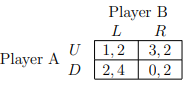
\includegraphics[scale=1.0]{Figure1.1}
	\end{center}
\end{enumerate}
% Question 3 Answers
\textcolor{gray}{
Answers:
\begin{enumerate}
	\setcounter{enumi}{2}
	\item To find all the Nash equilibria we will simply evaluate the best strategy for each player depending on which action the other player performs.\\\\
	So first evaluating player A's best strategy we know that if player B chooses column L then player A must choose row D because 2 is better than 1. If player B chooses coloumn R then playe rA's best choice would be to choose row U since 3 is greater then 0.\\\\
 	Now evaluating Player B's best stratey, we know that if player A chooses coloumn L then player B's best choice is to pick 
\end{enumerate}
}

% Question 4
\begin{enumerate}
	\setcounter{enumi}{3}
	\item  Consider the two-player game with players, strategies and payoffs described in the following game matrix.
	\begin{center}
		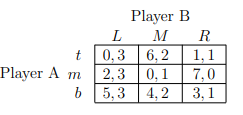
\includegraphics[scale=1.0]{Figure1.2}
	\end{center}
	\begin{enumerate}[(a)]
		% Question 4: Part 1
		\item Does either player have a dominant strategy? Explain briefly (1-3 sentences).
		% Question 4: Part 2
		\item Find all pure strategy Nash equilibria for this game.
	\end{enumerate}
\end{enumerate}
% Question 4 Answers
\textcolor{gray}{
Answers:
\begin{enumerate}
	\setcounter{enumi}{3}
	\item  Consider the two-player game with players, strategies and payoffs described in the following game matrix.
	\begin{enumerate}[(a)]
		% Question 4: Part 1
		\item Does either player have a dominant strategy? Explain briefly (1-3 sentences).
		% Question 4: Part 2
		\item Find all pure strategy Nash equilibria for this game.
	\end{enumerate}
\end{enumerate}
}

% Question 5
\begin{enumerate}
	\setcounter{enumi}{4}
	\item Consider the following two-player game in which each player has three strategies.\\
	\begin{center}
		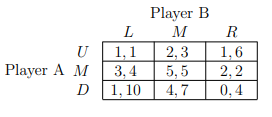
\includegraphics[scale=1.0]{Figure1.3}\\
	\end{center}
	Find all the (pure strategy) Nash equilibria for this game.\\
\end{enumerate}
% Question 5 Answers
\textcolor{gray}{
Answers:
\begin{enumerate}
	\setcounter{enumi}{4}
	\item Consider the following two-player game in which each player has three strategies.\\
	Find all the (pure strategy) Nash equilibria for this game.\\
\end{enumerate}
}
\end{document}
